\documentclass[FYP.tex]{subfiles}

\section{Developer Testing}

Whilst the software was being written, testing needed to be carried out to make sure that the system responded in the desired way. With a relatively short turn around time for the system development, an approach of Continuous Delivery was taken. This approach puts the user first and make sure that the software project is always in a presentable state to the user and a demo can be given. By writing code in this way, it meant that if time didn't allow to complete certain features, then it was not critical. This is because the code is always in a working state where it can be delivered to a user. This is important for a software project that needs to be tested not only by developers and experts, but also by casual users from the target audience. 

The Developer Testing consisted mainly of making a change to the system and directly testing that feature in the new version of the software. While testing in this way it is difficult to make sure that everything is working simultaneously. Responsibility lies with the developer to take the necessary procedures to make sure the software is working as required.

Constant sanity checks weremade to ensure that the software maintained all the core functionality. This included making sure that the rendering is correct, making sure the data structures were being represented correctly and making sure there was no runtime errors in the Javascript.  

Some of the requirements set out were to do with the code and the expansion of the project. Requirement \ref{ssection:nfun4} set out to make sure that the code was easily maintainable. This is obviously down to personal opinion but the effort has been made to fulfil this requirement. All of the function and variable names have been sensibly named, making the code easier to read. As well as this, the important pieces of code have been sufficiently commented, again giving guidance in how the code runs. Every function in the code has specific tasks to perform, like drawing the proof on the screen, but this results in some functions get large. Even though this has happened, because of good commenting of the code, it shouldn't be too hard to follow.

Requirement \ref{ssection:nfun5} set out that the code should be scalable. As features have been added to the software, the code has got more and more complex, leading to little intricacies. Whilst it not that difficult to add new levels to the game, significant logical changes will be difficult because of the way the code is structured. One of the main areas for improvement here that would allow for a more natural and aesthetically pleasing way to display larger proofs. The current way is perfect up to a proof height of 4 but finding a way to display larger proofs nicely would take a large step towards the software being scalable as it would comfortably allow much larger and complicated proofs to be displayed on the screen.

\section{Functional Testing}
\subsection{Unit Testing}

Unit testing is difficult to achieve in Javascript because of the nature of intertwined HTML and Javascript. Even so there are some functions which are stand alone and can be run without interference from any other function. These functions that run stand-alone can be tested to ensure that their behaviour is correct. To do this I created a new Javascript file and created a number of unit tests. These included tests for when objects are created and when objects are deleted. It analysed if objects were being created correctly and did a number of tests on the data structures to verify everything was working correctly. Results of the tests were printed out to the console, so the developer could analyse the results. The result of every subtest was logged to the console and if every subtask passed then the test passed. At the end of the testing, a summary was given saying how many tasks have passed and how many have failed. This gives a clear indication on whether all of the tested functionality is working correctly. When changes were made to the system, this would be the first check to make sure that all the tests have passed before undertaking the developer testing. Unfortunately, most of the other functionality of the code is difficult to be tested and therefore needed to be handled by the developer testing.

\subsection{Acceptance Testing}

Acceptance Testing is where testing is undertaken to decide whether the functional requirements set have been met by the implementation of the software. Asking the end users if they have had a successful and rewarding experience playing will go some way to deciding whether the requirements have successfully been implemented. Most functional requirements are straightforward and do not require user opinion on whether a certain targets or features have been implemented. This will be obvious to the developer, so analysis can be done internally to decide which functional requirements have been met.

Functional requirements were set in Section \ref{ssection:fun} and these will be dissected, with the the aim of explaining whether the requirement is met or not. The requirement \ref{ssection:fun1} is set out to 'Provide an intuitive drag and drop interface'. This has been achieved. Speaking to interested parties led to a change in how the drag and drop system works, meaning it has been improved and become more obvious. As previously mentioned in Section \ref{ssec:dots}, the drag and drop now works with a dots system. Being intuitive is obviously user dependent and in the event that users do not find the drag and drop intuitive, a tutorial has been created to explain to the users how everything works.

The HTML 5 creates a clear area where the user can drag and drop items. Users can drag all the elements that are created on the screen. The keyboard is not needed to be used for any part of the game which was prioritised in the implementation of the software. This successfully achieves requirement \ref{ssection:fun2}. By making everything drag and droppable, it lets the user do everything with the mouse, making is straightforward and simple.

Requirement \ref{ssection:fun3} was to have 'proofs rendered nicely so that they fit on the screen'. This was important so that users could see all parts of their proofs and view them clearly. For the levels that the user have to complete, all of the levels are rendered nicely. It has not yet been implemented that users can create proofs of infinite size all within the same box. The way the algorithm was structured did not make it possible to draw an infinite size proof in the same square. For large proofs, connecting squares are drawn which connect the leaves of the Natural Deduction tree together.

A free play mode has been implemented so that users can experiment with proofs and create them themselves. It is not possible for a user to create their own levels and any new levels need to be implemented by a developer. Future work could be to allow users the options to send the developers the levels they have created. The data structure could be captured and these could then be used to create more levels. Allowing users to experiment with proofs and letting users create their own levels was requirement  \ref{ssection:fun4} so this is partially fulfilled.

Requirement \ref{ssection:fun5} states that there should be a system that can successfully recognise whether a solution to a proof is correct. This has been achieved and the system will let the user know what part of the proof they have got wrong if they are incorrect. The ideal solution needs to be specified by the user and then the algorithm will go through each section of the proof to make sure it is correct.

Whilst facts can be given about what the software is capable of, recognition of whether the users feels gamification requirements have been successfully met will be shown in the results section of the project. 

The game has a hints box which successfully fulfils the requirement of \ref{ssection:fun6}. This hints box is available via a button at the bottom of the screen. Pressing this button loses the user 2 points from their score, but it is there to be helpful if possible. As well as this helpful hints box, learning prompts are displayed at the start of certain levels which teach the user how to accomplish certain tasks. A box containing the level goal clearly is located at the top of the screen. This tells the user the assumptions and the conclusions. This guides the user through levels as stated in requirement \ref{ssection:fun7}. Whilst all of these things aren't hints, they all give users clues about what they should be doing, contributing to the requirement of giving hints and tips to the user. There is also a tutorial at the beginning of the software which guides and helps the user through how to navigate the game.

There is points scoring system which gives the user points for each level depending on their achievements. This encourages the user to think for themselves about what they know before automatically going to the hints. This scoring system also informs the users in how well they are doing. This fulfils requirement \ref{ssection:fun8} and adds a competitive nature to the game where users can compare scores with each other.  

Requirement \ref{ssection:fun9} is that the game should be fun. This needs to decided by the user so this and other requirements will be set out in the results chapter where user feedback will be received.

     
\section{Non Functional \& Hardware Testing}
\subsection{Stress Testing}

Making sure that software can handle a number of users simultaneously is important for this project, as it is feasible that multiple users can log on to the webpage and play the game at the same time. The game is hosted on the University of Bath's servers, which process and hold a lot of data. Due to their industrial nature, I would assume that it would be able to deal with a lot of traffic and supporting users accessing the website at the same time wouldn't be an issue.

To test this theory, I used a load testing website that loaded 100 users onto the website and simulating them accessing the webpage simultaneously. \cite{loadTest} The results tested for load times and registered the number of successful virtual users on the site. Figure \ref{fig:stress} shows that 100 users successfully accessed the site simultaneously and that no load time for the webpage was above 1.5 seconds. This is a good achievement as a user will not be waiting a long time for the page to load. This shows the advantage of having all of the code client side, because it does not need to contact a server to retrieve the information once it has loaded for the first time, meaning that that waiting time will be the only waiting time in the entire game. Server side code may have a similar delay throughout the program. 

\begin{figure}[H]
\centering
\centerline{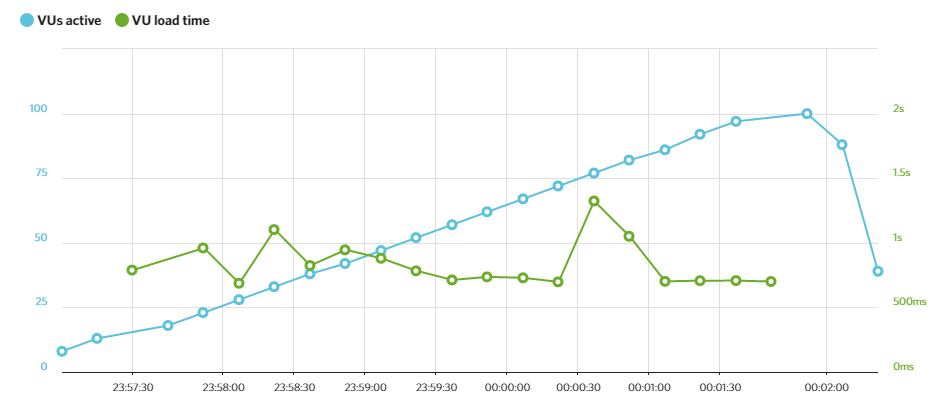
\includegraphics[scale=0.5]{StressTest}}
\caption{Load times and number of virtual users accessing the website over a period of 5 minutes}
 \label{fig:stress}
\end{figure}  

\subsection{Security Testing}

Security can be important to a lot of projects but in this project it is not too much of an issue. Sufficient security is in place that Javascript or HTML cannot be uploaded to the server or change permanently. This is another benefit to the whole of the code not needing to feed any information back to the server. If information was need to be uploaded to the server then there is some scope for inroads into the system.

Whilst it is not possible for the user to change the code in place that is stored on the server, because Javascript is being used it means that users can have access to the whole code base. This means that if the users really wanted to then they could find the answers that are scored in the code to complete the levels. Whilst this against the spirit of the game, as it is meant to act as an educational tool, it is possible to circumnavigate the system in this way. This level of security that the code cannot be changed permanently fulfils requirement \label{ssection:nfun3}.

\subsection{Compatibility Testing}

As this is web software, requirements to make sure that it will work on a variety of different browsers, different operating systems and different architectures.  This requirement was set out by \ref{ssection:hard2}. The code is not very demanding so it should be capable of working on even basic architectures. The only problem that may be encountered would be if the web browser doesn't support a HTML 5 canvas. Research was undertaken to make sure this requirement was fulfilled. The code was written on a Windows laptop running Windows 10 OS and an AMD processor. On this laptop, the website was loaded on Chrome, Firefox and Internet Explorer and it all worked fine. An online resource outlines which web browsers support a HTML 5 canvas stated that a HTML canvas is supported by all current versions of Microsoft Edge, Google Chrome and Mozilla Firefox. It is also supported by Internet Explorer 9 onwards, but the canvas not supported by IE8. The website goes on to state that the HTML5 canvas is accessible to approximately 94.38\% of UK users, based on statistics about the browsers that are used in the UK. \cite{CanIu61:online}     

\subsection{Other Hardware Comments}

By using a combination of HTML and Javascript for the software, it naturally achieves Requirement \ref{ssection:hard1}. This means all the code is loaded onto the client's web browser and as shown in ref{fig:stress}, means that loading times are fairly small. These are the only loading times in the game because the server doesn't need to be contacted for more information. This leads to quick response times and smooth gameplay.

This software is naturally compatible with a PC or Laptop. Currently, it is not available to play on a touchscreen and this would be one of the main features that could be implemented in improvements to the software. Making the software native to a PC and Laptops realises requirement \ref{ssection:hard3}. Because of what was set out in the requirements, it was always planned to implement the software for mobiles at a later date. 

\cite{Softw57:online}